\begin{abstract}
Max flow algorithms have improved a lot since the paper by L. R. Ford and D. R. Fulkerson in 1956 \cite{FordFulkerson}.
The most recent contribution by Orlin \cite{Orlin13} shows that all instances can be solved in $O(nm)$ time.
In this thesis, we will outline the history of max flow problems, as well as implement and compare some of the most interesting ones.
In an effort to improve performance, we managed to reduce the memory used by an algorithm by V. King and S. Rao \cite{King1992} from $O(nm)$ to $O(m)$, 
without compromising the theoretical running time.
\end{abstract}

\clearpage

\section{Introduction}
The max flow problem is a directed graph problem. A graph consists of a set of nodes and a set of edges connecting the nodes.
The edges are directed, meaning that if an edge goes from the node $v_i$ to the node $v_j$, you will be able to follow that edge from $v_i$ to $v_j$, but not the other way.
The graph contains two special nodes, a \emph{source} node $s$ and a \emph{target} node $t$.
The problem is to determine how much flow can be sent through the graph from $s$ to $t$.
Each edge has a limit to the amount of flow that you can send over that edge. 
This limit is called the capacity of the edge, and that is what limits how much flow that you can send from $s$ to $t$.
In the end of any max flow algorithm, there is not allowed to be any flow imbalance in nodes other than $s$ and $t$.
That means that for any node other than $s$ and $t$, the total amount of incoming flow has to be equal to the total amount of outgoing flow.
An example can be seen in Figure~\ref{maxFlowExample}. The numbers on the edges in the first graph signify the capacity of the edges.
The numbers in the solution graph signify how much flow is sent on the edge out of the capacity on the edge.
\begin{figure}[ht!]
\centering
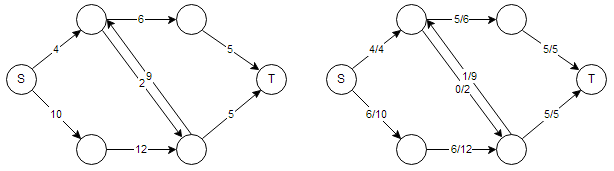
\includegraphics[width=90mm]{MaxFlowExample.png}
\caption{An example of a max flow problem and a solution to it}
\label{maxFlowExample}
\end{figure}

A number of problems can be reduced to the max flow problem, such as maximum cardinality bipartite matching, maximum independent path and maximum edge-disjoint path.
Maximum cardinality bipartite matching problem is, given a bipartite undirected graph with node sets $U$ and $V$, 
select the maximum number of edges connecting $u\in U$ and $v \in V$ such that no nodes are connected to two selected edges.
An example of using max flow to solve maximum cardinality bipartite matching can be seen in Figure~\ref{maxCardinalityBipartiteMatchingExample}.
\begin{figure}[ht!]
\centering
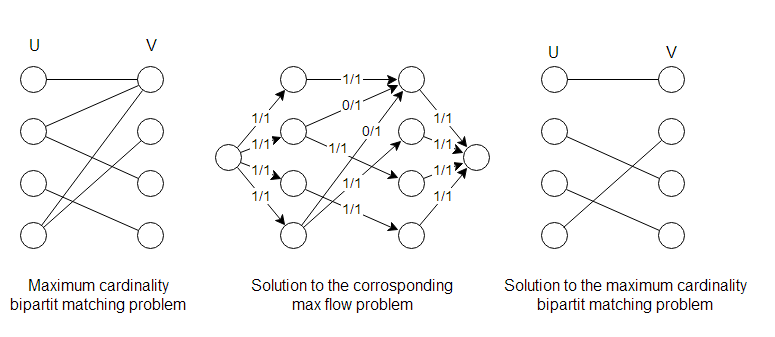
\includegraphics[width=90mm]{MaxCardinalityBipartitMatchingExample.png}
\caption{A max flow solution to maximum cardinality bipartite matching}
\label{maxCardinalityBipartiteMatchingExample}
\end{figure}



An area where real world max flow problems arise is in computer vision. 
The problem of identifying objects in an image can be reduced to a min-cut problem, which is the dual of the max flow problem.
Min cut being the dual of the max flow means that solutions to one of the problems can easily be transformed into a solution to the other.
Furthermore, making a cut in the graph gives an upper bound to the solution while a valid flow in the graph is a lower bound on the solution.

Max flow algorithms have been around since 1956 \cite{FordFulkerson}, and since then many interesting algorithms have been published in the field.
A recent publication by Orlin \cite{Orlin13} proved that max flow problems can be solved in $O(nm)$ time for sparse graphs where $m=O(n^{16/15-\varepsilon})$.
Combined with a result by V. King and S. Rao \cite{King1992}, this means that we have an $O(nm)$ time algorithm for all max flow problems.

Many of the max flow algorithms focus on providing theoretical improvements, and have little to no focus on practical running time.
In this thesis, we will compare the practical running time on a selected subset of the max flow algorithms.
We have decided only to consider max flow problems with integer capacities. The reason for this is that it makes it simpler to implement the algorithms if we don't have to take floating point errors into account.
With integer capacities, all correct implementations are guaranteed to return exactly the same output, which makes it easier to verify.

We start by going over the terminology that we will use throughout the thesis in Section~\ref{TerminologySection}.
Some central ideas are repeated throughout several papers. We give a general overview of these ideas in Section~\ref{ParadigmsSection}.
Section~\ref{SurveySection} will contain a survey where we give a brief overview of the main improvements made since the first paper in the field \cite{FordFulkerson}.
Sections~\ref{EK1972Section} to~\ref{GRSection} contain more detailed descriptions of the algorithms we selected to study. 
We explain how the algorithms work, how they achieve their bounds, and what, if any, modifications we have done to implement them.
Sections~\ref{TestsSection} and~\ref{ResultsSection} contain a description of the tests we have run, and the results we have obtained.